\documentclass[12pt]{article}
\usepackage[utf8]{inputenc}
\usepackage{graphicx}
\usepackage{geometry}
\geometry{a4paper, margin=1in}

\title{Assignment 3 -- MLflow Experiment Report}
\author{Ahmed}
\date{March 10, 2026}

\begin{document}

\maketitle

\section{Table View}
All 5 runs sorted by \texttt{test\_accuracy} (highest first).

\begin{figure}[h]
    \centering
    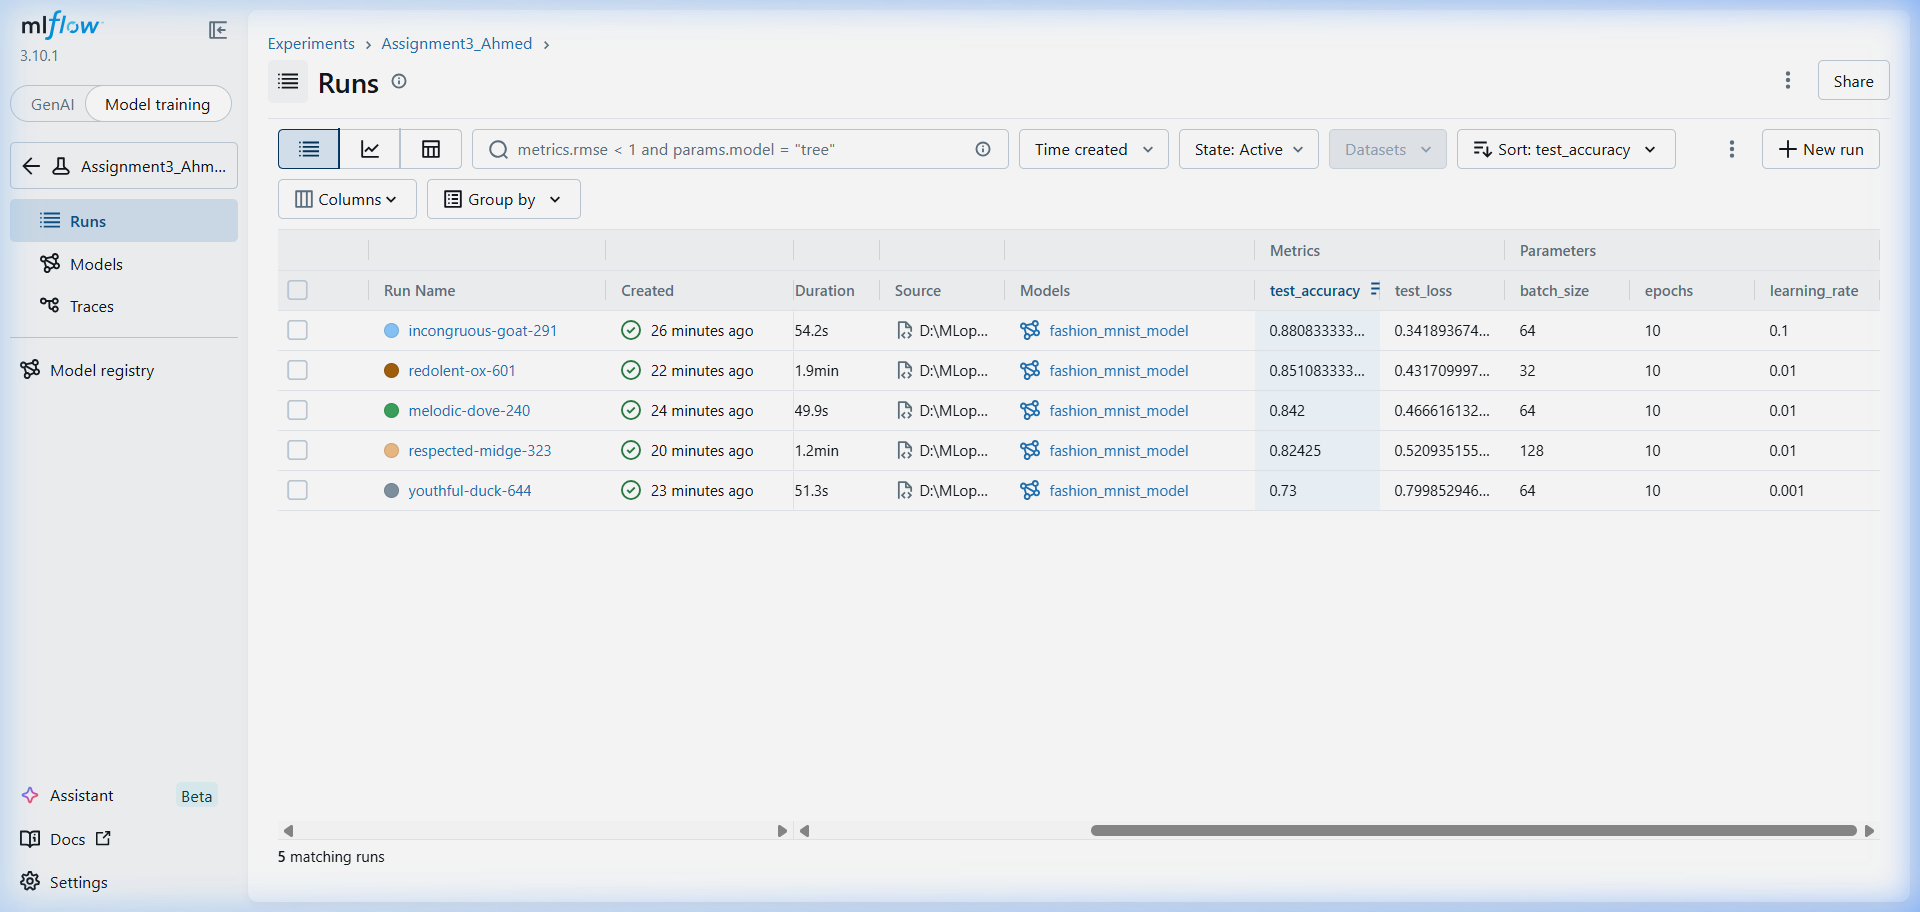
\includegraphics[width=\textwidth]{mlflow_table_view.png}
    \caption{Table View -- 5 runs sorted by test\_accuracy.}
\end{figure}

\section{Comparison View}
Training accuracy curves for all 5 runs overlaid on one chart.

\begin{figure}[h]
    \centering
    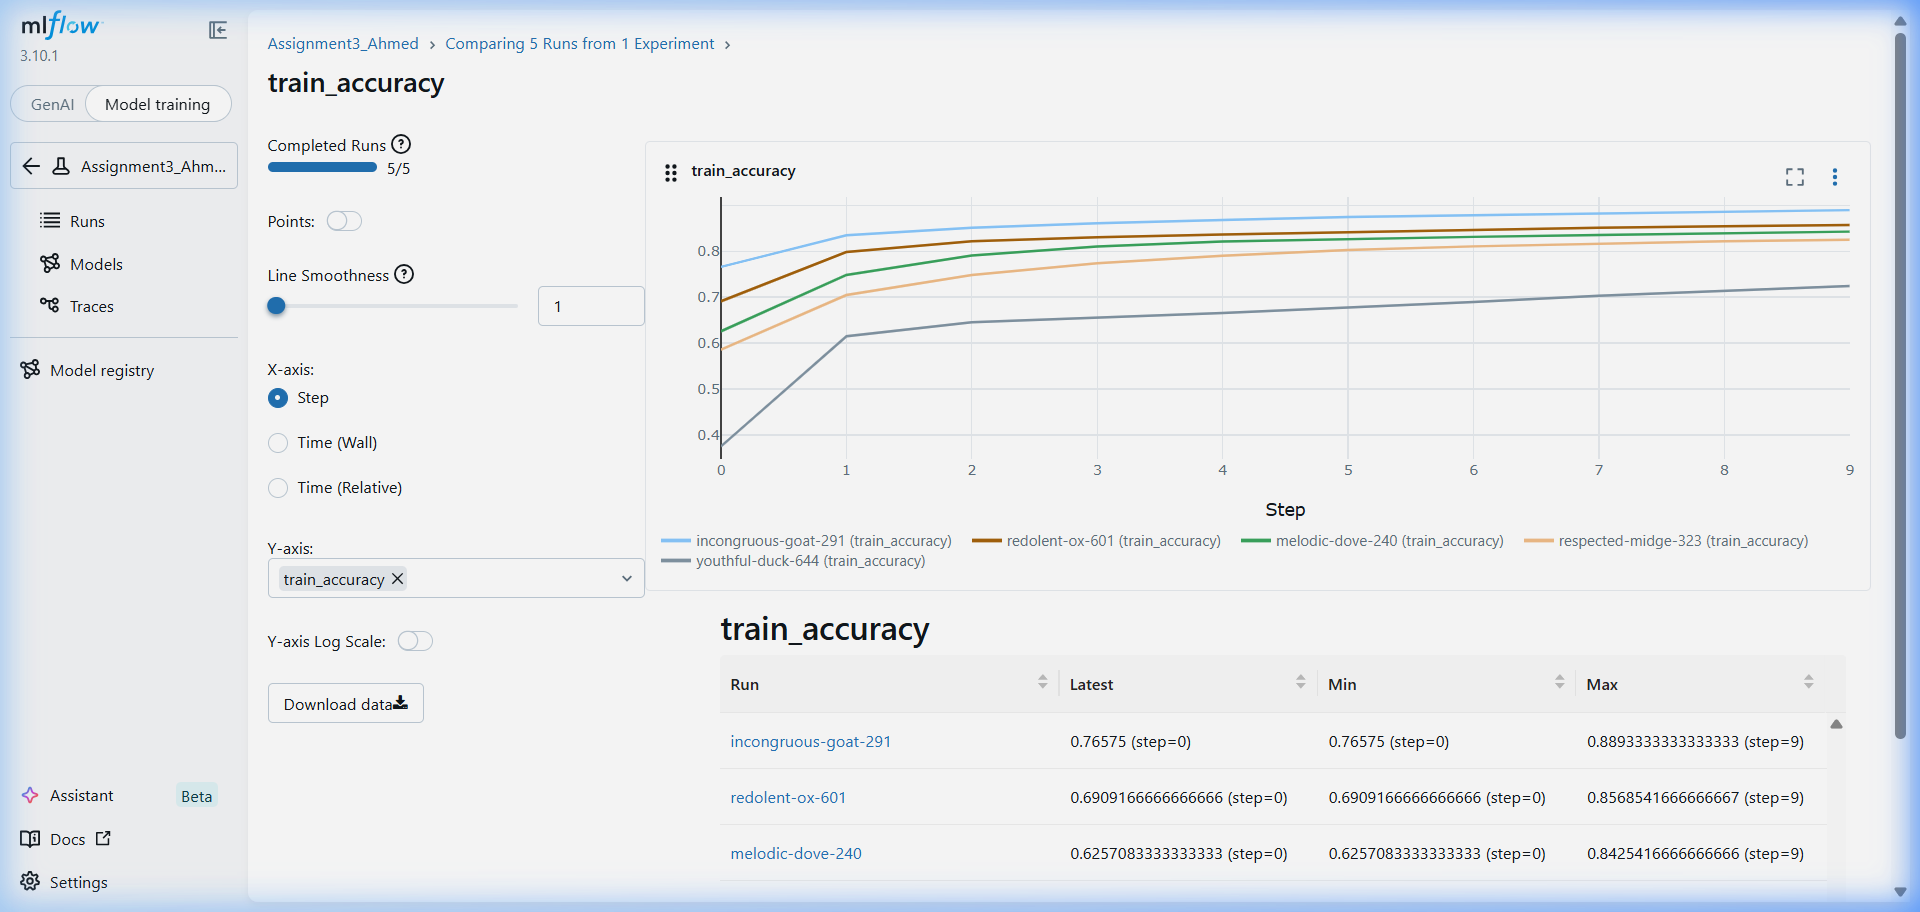
\includegraphics[width=\textwidth]{mlflow_comparison_view.png}
    \caption{Comparison View -- train\_accuracy curves overlaid.}
\end{figure}

\section{Artifact Gallery}
Artifacts tab showing saved model, MLmodel metadata, and environment files.

\begin{figure}[h]
    \centering
    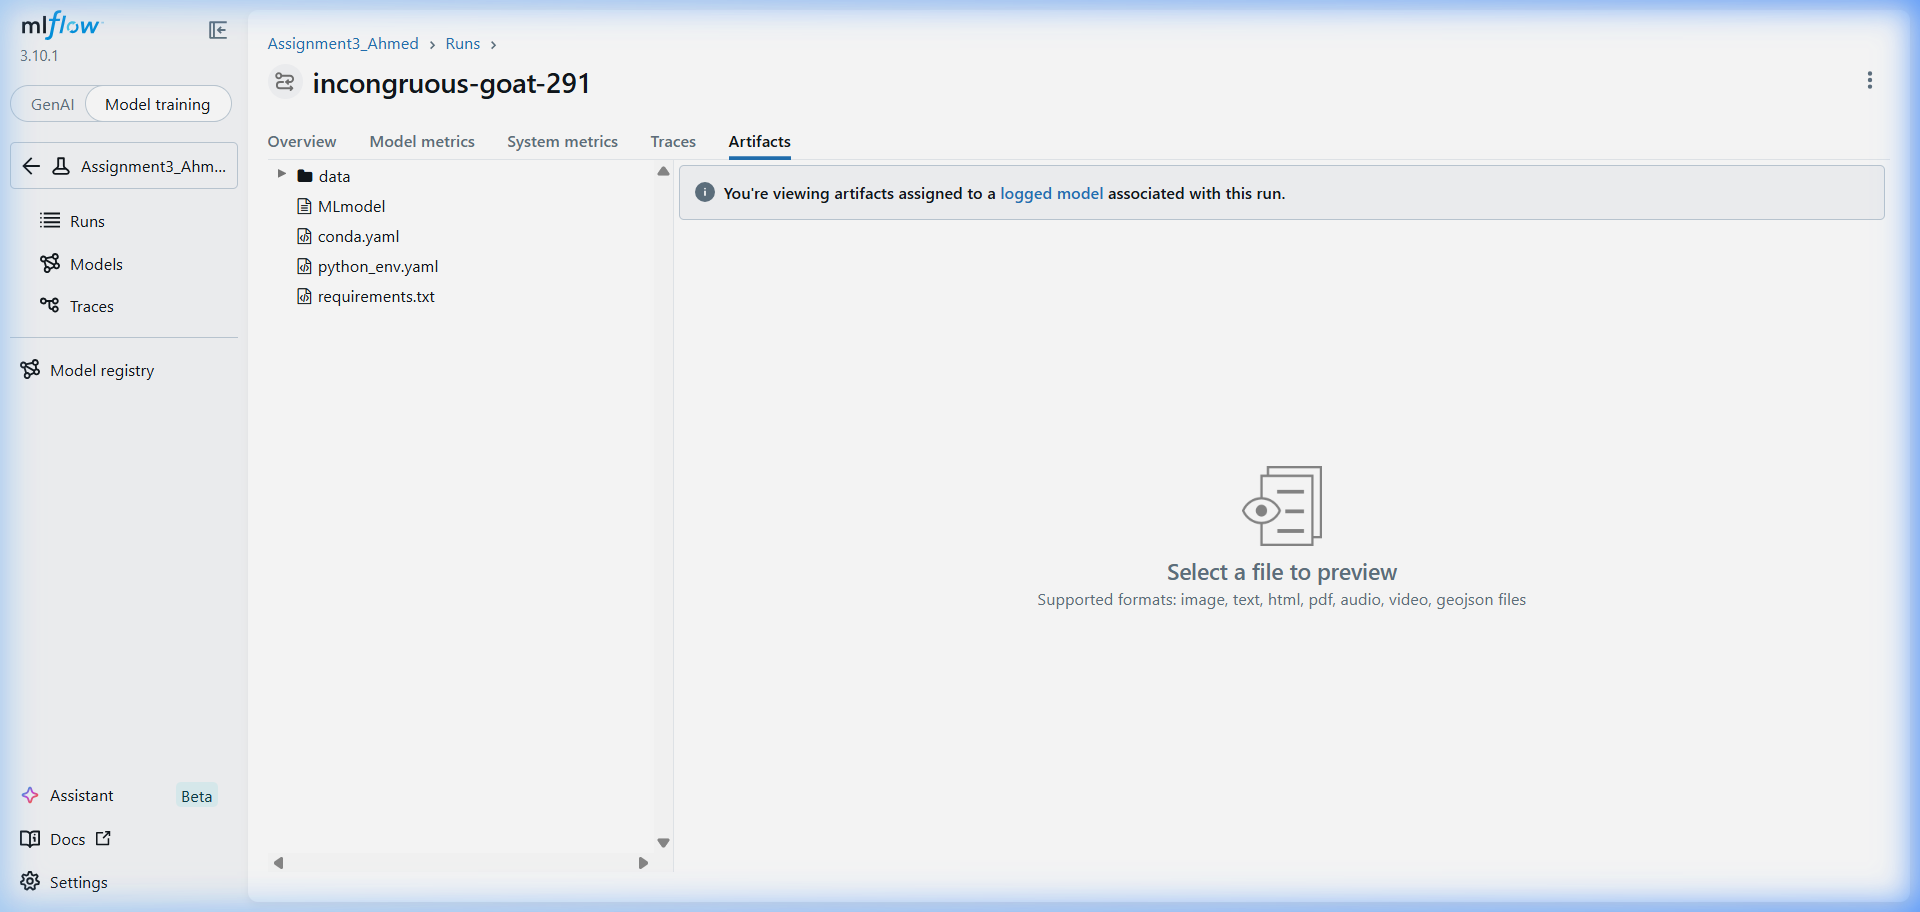
\includegraphics[width=\textwidth]{mlflow_artifacts_view.png}
    \caption{Artifact Gallery -- model and environment files.}
\end{figure}

\section{Short Analysis}

\begin{itemize}
    \item \textbf{Winner:} The run with \texttt{lr=0.1, batch\_size=64} achieved the highest test accuracy of \textbf{88.08\%} and the lowest test loss of \textbf{0.3419}.

    \item \textbf{Underfitting:} The run with \texttt{lr=0.001} clearly underfits with only \textbf{73\%} test accuracy. The learning rate is too small to converge in 10 epochs.

    \item \textbf{Overfitting:} No severe overfitting was observed. Training and test accuracies were close for all runs.

    \item \textbf{Batch size effect:} Among the \texttt{lr=0.01} runs, \texttt{batch\_size=32} gave the best result (85.1\%), followed by \texttt{batch\_size=64} (84.2\%), then \texttt{batch\_size=128} (82.4\%). Smaller batches gave better accuracy.
\end{itemize}

\end{document}
